\subsection{IPv6 hierarchical address allocation}\label{sec:mhcl}

MHCL partitions the address space available to the border router, for instance the 64 least-significant bits of the IPv6 address (or a compressed 16-bit representation of the latter), hierarchically among nodes connected to the border router through a multihop cycle-free topology (implemented by standard protocols, such as RPL~\cite{rfc6550} or CTP~\cite{Fonseca:2009}). Each node
receives an address range from its parent and partitions it among its children, until all nodes receive an address (see Figure \ref{fig:mhcl}). Since the address allocation is performed in a hierarchical way, the routing table of each node can have $k$ entries, where $k$ is the number of its (direct) children. Each routing table entry aggregates the addresses of all nodes in the subtree rooted at the corresponding child-node. However, MHCL does not handle tree topology dynamics, i. e., a failure on a node or link can cause some local topology changes, which can break the hierarchical nature of MHCL. In \cite{mhcl}, only packet loss were handled. Therefore, it is necessary to design a mechanism to cope with local topology changes able to maintain routing with low memory footprint.

\begin{figure}[!ht]
    \centering
    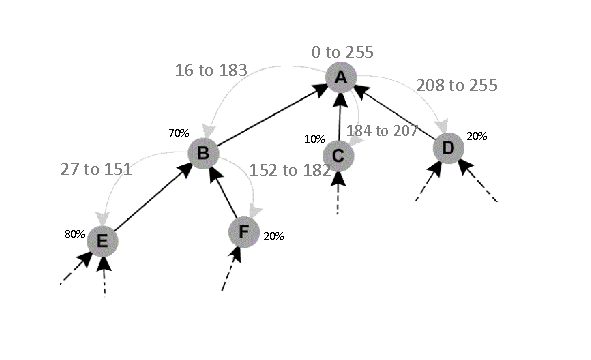
\includegraphics[width=1\linewidth]{./Images/mhcl.pdf}
\caption{Example of MHCL address assignment. 8-bit address space at the root and $6.25\%$ of address range reserved for future/delayed connections}
    \label{fig:mhcl}
\end{figure}

In order to decide how the available address space is partitioned, nodes need to collect information about the topology of the network. To do this, each node $n_i$ counts the total number of its descendants, i.e., the size of the subtree rooted at itself, and propagates it to its parent. Moreover, $n_i$ saves the number of descendants of each child. Once the root has received the number of descendants of each child, it partitions the available address space into $k$ slices of size proportional to the size of the subtree rooted at each child, also leaving a portion of $r\%$ as reserve. Each node $n_i$ repeats the space partitioning procedure upon receiving its own address space from the parent and sends the proportional address slices to the respective children. The idea is to allocate larger address portions to larger subtrees, which becomes important in especially large networks, because it maximizes the address space utilization. Experiments in \cite{mhcl} shown that MHCL is efficient in number of messages and time. Nevertheless, due to simulations' constraints, the results were not satisfactory and only few scenarios were evaluated. In addition, there were a lot of dependency between the proposed protocol and RPL, which can affect the results.